\section{Trust Regions for Policy Gradients }
One problem that arises with policy gradients methods is that the distance in 
parameter space does not translate into policy space. As a result, small changes in 
the parameters can lead to a large changes in policy behaviour. This could even go 
so far as to make our policy so bad that we cannot recover from it. A popular method 
is to limit the difference between subsequent policies to increase stability.

\subsection{Trust regions}
To ensure that the difference between subsequent policies remains limited, we can reformulate the general
objective of maximizing with respect to both the previous and current policies as we did in section \ref{data_reuse}.
This formulation includes an additional constraint to prevent large differences between consecutive policies which 
is achieved by limiting a dissimilarity measure  $D(\cdot,\cdot)$ (i.e. Kullback-Leibler divergence) between the distributions:
\begin{gather*}
\theta_{\text{new}} = \argmax\limits_\theta \mathbb{E}_{(s,a)\sim \pi_{\text{old}}}\left[\frac{\pi_{\theta}(a|s)}{\pi_{\text{old}}(a|s)} A^{\pi_{\text{old}}}(s,a)\right] \qquad  
\text{s.t. } D(\pi_\theta(a|s),\pi_{\text{old}}(a|s)) \leq \epsilon, \forall s \in S
\end{gather*}
We now have a constrained optimization problem that requires specialized methods for solving, which we will look at next.

\subsection{Lagrangian Multipliers}\label{lagrangian_multipliers}
We start by introducing the following optimisation problem:
$$ \underbrace{\min\limits_x f(x)}_{\text{objective}} \qquad \text{s.t } 
\underbrace{h_i(x) \geq b_i, \text{ for } i=1\dots K}_{\text{constraints}}$$
We then define the Lagrangian function/ Lagrangian , which combines the objective and constraint into a single function:
$$ L(x,\lambda) = f(x)- \underset{i=1}{\sum^K}\lambda_i(h_i(x)-b_i) \quad \text{s.t. } \lambda_i \geq 0, \text{ for } i= 1\dots K$$
We call the $\lambda_i$ the Lagrange multipliers. There are now two ways how we can solve this problem in order to solve our original 
optimization problem :
\vspace{-1.2cm}
\begin{multicols}{2}
   \begin{gather*}
      \textbf{Primal optimization problem} \\
      \min\limits_x \max\limits_\lambda L(x,\lambda) 
  \end{gather*}\break
  \begin{gather*}
      \textbf{Dual optimization problem} \\
      \lambda^* = \argmax\limits_\lambda g(\lambda), \qquad g(\lambda)=\min\limits_x L(x,\lambda)
  \end{gather*}
\end{multicols}
The question now is: which problem should we choose to solve, and do we actually obtain the optimal solutions through 
this approach?\newline
The solutions of the primal problem also minimize the unconstrained objective. However, solving the primal problem can
often be challenging, especially since it might not possess the necessary convexity properties, making it hard to solve
directly. But what about the dual function?\newline
Since $ g(\lambda) $ is a pointwise minimum of affine functions (note that $ \mathcal{L}(x, \lambda) $ is affine in $ \lambda $,
even though $ f(x) $ might not be linear or affine but we treat it as a constant with respect to $ \lambda $), the dual function 
is concave (see the proof \cite{Proof_Lagrangian_Concave}). Since $ g(\lambda) $ is concave 
and the constraints are linear (meaning they are convex), maximizing $ g(\lambda) $ over $ \lambda $ is a convex optimization problem. 
Furthermore, because convex functions have the property that every local minimum is also a global minimum, it is easier to solve using 
standard optimization techniques than the primal problem.\newline
But what can we say about the solutions from both methods? Any feasible solution to the primal problem is at least as large 
as any feasible solution to the dual problem. Therefore, the solution to the primal provides an upper bound to the solution 
of the dual, and the solution of the dual provides a lower bound to the solution of the primal. This fact is known as 
\textbf{weak duality}:
$$
g(\lambda) = \min_{x} \mathcal{L}(x, \lambda) \leq \min_{x} f(x) = p^* \quad \Rightarrow \quad d^* = \max_{\lambda} g(\lambda) \leq p^*
$$
In general the optimal values of the primal and dual problems, $ p^* $ and $ d^* $ do not need be equal. The difference between them 
is called the \textbf{duality gap}.
\subsubsection{Lagrangian Multipliers cookbook}
\begin{enumerate}
    \item Write down Langrangian  $L(x,\lambda) = f(x)- {\sum_{i=1}^K}\lambda_i(h_i(x)-b_i)$
    \item Obtain optimal solution for primal parameters (primal solution) $\frac{\text{d}L(x,\lambda)}{\text{d}x} = 0 
    \rightarrow x^* = u(\lambda)$
    \item put $x^*$ back into the Lagrangian $g(\lambda) = L(u(\lambda),\lambda)$
    \item obtain optimal solution for $g(\lambda) \rightarrow \lambda^* = \argmax\limits_\lambda g(\lambda), 
    \text{ s.t. } \lambda_i \geq 0 \;\forall i$
    \item $x^* = u(\lambda^*)$
\end{enumerate}
An important aspect of using the Lagrangian is how to construct it, depending on the type of optimization problem and constraints.
Consider the following simple example:
\begin{gather*}
    \min\limits_x x^2 \text{ s.t. } x\geq1 \longrightarrow L(x,\lambda)= x^2 - \lambda(x-1)
\end{gather*}
The Lagrangian must be constructed in such a way that violating the constraint will not lead to an optimal solution.
Since Lagrange multipliers are non-negative (i.e., $\lambda \geq 0$), violating the constraint $x \geq 1$ would result in adding a positive 
term, even though the goal is to minimize the objective function. This ensures that when $x < 1$ the Lagrangian penalizes this violation,
and vice versa for a maximization problem. To gain a deeper understanding, let’s now consider a more complex example.
\begin{gather*}
  \underset{\boldsymbol{\omega}}{\textrm{argmax}} \int p_{\boldsymbol{\omega}}(\boldsymbol{\theta})g(\boldsymbol{\theta}) 
  d\boldsymbol{\theta} \quad \textrm{s.t.} \quad \textrm{KL}(p_{\boldsymbol{\omega}}(\boldsymbol{\theta}) || p_{\textrm{old}}
  (\boldsymbol{\theta})) \leq \epsilon, \quad \textrm{H}(p_{\boldsymbol{\omega}}(\boldsymbol{\theta})) \geq \beta, \quad \int 
  p_{\boldsymbol{\omega}}(\boldsymbol{\theta}) d \boldsymbol{\theta}=1.
\\
\rightarrow L(p_w,\eta,\kappa) = \int p_w(\theta)g(\theta)d\theta + \eta \left(\epsilon - \textrm{KL}(p_w(\theta)||p_{\textrm{old}}(\theta))\;\right)+\kappa (\textrm{H}(p_w(\theta))-\beta) + \lambda \left( \int p_w(\theta)d\theta -1\right)
\end{gather*}
Notice how we now use $+$ instead of $-$ because this is a maximization problem. And try verifying for yourself, for each of the constraints,
what the outcome (in terms of sign) would be if they were violated. Does this help or penalize in finding the optimal solution?

 \subsection{Trust Region Policy Optimization (TRPO)}
 One of the first methods to introduce this idea of constraining the update step was TRPO  \cite{schulman2017trustregionpolicyoptimization}. The objective is defined as follows 
 \begin{align*}
     \max\limits_{\pi} J(\theta) = \mathbb{E}_{(s,a) \sim \pi_{\text{old}}} 
     \left[\frac{\pi_{\theta}(a|s)}{\pi_{\text{old}}(a|s)} A^{\pi_{\text{old}}}(s,a)\right] \qquad
     \text{Constraint: s.t.: } \mathbb{E}_{\pi_{\text{old}}}\left[\text{KL}(\pi_{\theta}|\pi_{\text{old}})\right] \leq \epsilon
 \end{align*}
In order to derive the update step the TRPO Paper uses something called the Natural-Gradient.
In standard gradient-based optimization, we use the gradient of the objective function with respect to the parameters to update the model. However, this method treats all
directions in parameter space as if they are equally important, which may not be the case since parameters in different 
regions may have different scales/curvatures leading to inefficient learning/bad model performance.\newline The natural gradient 
takes into account the geometry of the parameter space. It adjusts the gradient by scaling it with respect to the ''natural``
metric, which is defined by the Fisher information matrix (a matrix that measures the sensitivity of the model's output with 
respect to its parameters).\newline
Natural gradients use a Taylor expansion approximation of the trust region problem
\begin{gather*}
{\mathcal L}(\theta_k, \theta) \approx \nabla_\theta J(\theta)^T (\theta - \theta_k) \\  \\
\bar{D}_{KL}(\theta || \theta_k)  \approx \frac{1}{2} (\theta - \theta_k)^T F (\theta - \theta_k) \qquad \underbrace{F =\frac{\text{d KL}
(\pi_\theta||\pi_{\theta_{\text{old}}})}{\text{d}\theta\text{d}\theta} =\underset{\pi_\theta}{\mathbb{E}}[\nabla_\theta \log{\pi_\theta(a|s)}
{\nabla_\theta \log{\pi_\theta(a|s)}}^T]}_{\text{Fisher information matrix}}
\end{gather*}
This approximate problem can be analytically solved by the methods of Lagrangian duality, yielding the solution:
$$\theta_{k+1} = \theta_k + \sqrt{\frac{2 \epsilon}{{\nabla_\theta J(\theta)}^T F^{-1} \nabla_\theta J(\theta)}} F^{-1} \nabla_\theta J(\theta).$$
There is one small issue with this approach when implemented naively: it concerns storing the inverse of the Fisher information matrix. Since 
the matrix $F$ is $|\theta|\times|\theta|$ dimensional, it would require excessive memory for a neural network with millions of parameters.
TRPO sidesteps the issue by using the conjugate gradient algorithm to solve $Fx =  \nabla_\theta J(\theta)$ for $x = F^{-1}  \nabla_\theta 
J(\theta)$, requiring only a function which can compute the matrix-vector product $Fx$ instead of computing and storing the whole matrix $F$ 
directly.
\begin{algorithm}[H] 
\caption{TRPO (OpenAI’s Spinning Up version \cite{OpenAI_Spinning_UP})} 
\label{algo:trpo} 
\begin{algorithmic} 
\STATE Input: initial policy parameters $\theta_0$, initial value function parameters $\phi_0$ 
\STATE Hyperparameters: KL-divergence limit $\delta$, backtracking coefficient $\alpha$, maximum number of backtracking steps $K$ 
\FOR{$k = 0,1,2,...$} 
\STATE Collect set of trajectories ${\mathcal D}_k = \{\tau_i\}$ by running policy $\pi_\text{old} = \pi(\theta_k)$ in the environment. 
\STATE Compute rewards-to-go $\hat{R}_t$. 
\STATE Compute advantage estimates, $\hat{A}_t$ (using any method of advantage estimation) based on the current value function $V_{\phi_k}$. 
\STATE Estimate policy gradient as 
\begin{equation*} \hat{g}_k = \frac{1}{|{\mathcal D}_k|} \sum_{\tau \in {\mathcal D}_k} \sum_{t=0}^T \nabla_\theta \frac{\pi_{\theta}(a_t|s_t)}{\pi_{\text{old}}(a_t|s_t)} A^{\pi_{\text{old}}}(s_t,a_t)
%\left. \nabla_{\theta} \log\pi_{\theta}(a_t|s_t)\right|_{\theta_k} \hat{A}_t. 
\end{equation*} 
\STATE Use the conjugate gradient algorithm to compute 
\begin{equation*} \hat{x}_k \approx \hat{H}_k^{-1} \hat{g}_k, \end{equation*}
where $\hat{H}_k$ is the Hessian of the sample average KL-divergence. 
\STATE Update the policy by backtracking line search with \begin{equation*} \theta_{k+1} = \theta_k + \alpha^j \sqrt{ \frac{2\delta}
{\hat{x}_k^T \hat{H}_k \hat{x}_k}} \hat{x}_k, \end{equation*} where $j \in \{0, 1, 2, ... K\}$ is the smallest value which improves the 
sample loss and satisfies the sample KL-divergence constraint. 
\STATE Fit value function by regression on mean-squared error: \begin{equation*} \phi_{k+1} = \arg \min_{\phi} \frac{1}{|{\mathcal D}_k| T} 
\sum_{\tau \in {\mathcal D}_k} \sum_{t=0}^T\left( V_{\phi} (s_t) - \hat{R}_t \right)^2, \end{equation*} typically via some gradient descent 
algorithm. 
\ENDFOR 
\end{algorithmic} 
\end{algorithm}

\subsection{Proximal Policy Optimization (PPO)}
PPO \cite{schulman2017proximalpolicyoptimizationalgorithms} is another method that incorporates the idea of trust regions. There are two main variants: PPO-Penalty and PPO-Clip. We will focus  
here only on PPO-Clip.\newline 
PPO-Clip does not rely on an explicit dissimilarity measure between policies. Instead, it controls the difference between successive 
policies using a clipping mechanism and a min function, which are built directly into the loss function.
\begin{gather*}
\theta_{k+1} = \arg \max_{\theta} \underset{s,a \sim \pi_{\theta_k}}{{\mathrm E}}\left[L(s,a,\theta_\text{old}, \theta)\right] \\
L(s,a,\theta_\text{old},\theta) = \min\left(
\frac{\pi_{\theta}(a|s)}{\pi_{\theta_\text{old}}(a|s)}  A^{\pi_{\theta_\text{old}}}(s,a), \;\;
\text{clip}\left(\frac{\pi_{\theta}(a|s)}{\pi_{\theta_\text{old}}(a|s)}, 1 - \epsilon, 1+\epsilon \right) A^{\pi_{\theta_\text{old}}}(s,a)
\right),
\end{gather*}
As stated in the original PPO-Paper \cite{schulman2017proximalpolicyoptimizationalgorithms} : ''$\dots$The second term (clipped ratio), 
modifies the objective by clipping the probability ratio, which removes the incentive for moving it outside of the interval 
$[1-\epsilon,1+\epsilon]$. Finally, we take the minimum of the clipped and unclipped objective, so the final objective is a 
lower bound (i.e. a pessimistic bound) on the unclipped objective. With this scheme, we only ignore the change in probability 
ratio when it would make the objective improve, and we include it when it makes the objective worse ``.
The intuition for the clipping can be best seen in figure \ref{ppo_lclip}. 
\begin{figure}[H]
    \centering
    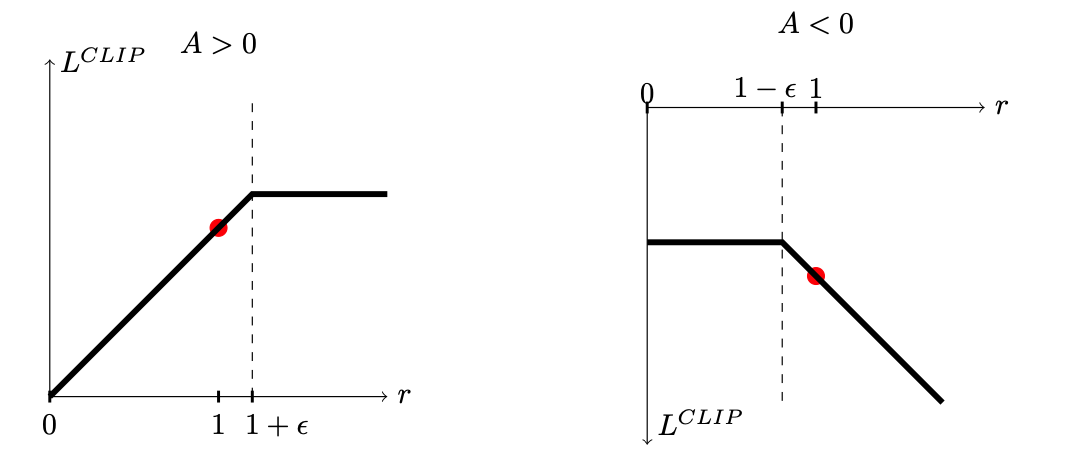
\includegraphics[width=0.8\linewidth]{images/ppo_lclip.png}
    \caption{Plots showing one term (i.e a single timestep) of the surrogate function $L$ as a function of the probability ratio $r$, for positive advantages left and negative advantages right, from \cite{schulman2017proximalpolicyoptimizationalgorithms}}
    \label{ppo_lclip}
\end{figure}
When the advantage is positive meaning the action we took lead to a better value then we would want the
policy to do more of this actions but the clipping in this case lets us not go beyond the $1+\epsilon$ ratio. When 
the advantage is negative meaning the action was less than favourable then there has to be at minimum a punishment of 
$1-\epsilon$ but there is no lower bound to it. 
\begin{algorithm}[H] 
\caption{PPO-Clip (OpenAI’s Spinning Up version \cite{OpenAI_Spinning_UP})} \label{alg:PPO-Clip} 
\begin{algorithmic} 
\STATE Input: initial policy parameters $\theta_0$, initial value function parameters $\phi_0$ 
\FOR{$k = 0,1,2,...$} 
\STATE Collect set of trajectories ${\mathcal D}_k = \{\tau_i\}$ by running policy $\pi_\text{old} = \pi(\theta_k)$ in the environment. 
\STATE Compute rewards-to-go $\hat{R}_t$. 
\STATE Compute advantage estimates, $\hat{A}_t$ (using any method of advantage estimation) based on the current value function $V_{\phi_k}$. 
\STATE Update the policy by maximizing the PPO-Clip objective: 
\begin{equation*} \theta_{k+1} = \arg \max_{\theta} \frac{1}{|{\mathcal D}_k| T} \sum_{\tau \in {\mathcal D}_k} \sum_{t=0}^T 
\min\left( \frac{\pi_{\theta}(a_t|s_t)}{\pi_{\theta_\text{old}}(a_t|s_t)} A^{\pi_{\theta_\text{old}}}(s_t,a_t), \;\; g(\epsilon, A^{\pi_{\theta_\text{old}}}(s_t,a_t))
\right), 
\end{equation*} typically via stochastic gradient ascent with Adam. 
\STATE Fit value function by regression on mean-squared error: 
\begin{equation*} \phi_{k+1} = \arg \min_{\phi} \frac{1}{|{\mathcal D}_k| T} \sum_{\tau \in {\mathcal D}_k} \sum_{t=0}^T\left( V_{\phi} (s_t) - \hat{R}_t \right)^2, 
\end{equation*} typically via some gradient descent algorithm. 
\ENDFOR \end{algorithmic} \end{algorithm}
PPO shows very impressive results, but there are many additional hacks needed to make it really perform well,
to list some: Value function clipping, Reward scaling, orthogonal initialisation, Adam learning rate annealing, reward clipping, 
observation normalisation, observation clipping, hyperbolic tan activations, Global gradient clipping

\subsection{Differentiable Trust Region Layers}
Recent work has shown that convex optimization problems can be embedded as differentiable layers within neural 
networks \cite{agrawal2019differentiableconvexoptimizationlayers}, enabling end-to-end training through optimization-
based components. Building on this idea, differentiable trust region layers enforce trust region constraints directly 
within the policy network \cite{otto2021differentiabletrustregionlayers}. This transforms what would otherwise be a 
complex constrained optimization problem into a standard differentiable layer that integrates seamlessly into deep 
reinforcement learning pipelines.

\subsection{Maximum Posteriori Optimization (MPO)}
MPO is the idea of Trust-Regions for Actor Critic Methods. MPO uses 2 steps to optimize the policy (inspired by Expectation Maximization)
\begin{itemize}
\item E-Step: Solve Trust Region problem for non-parametric distribution
\item M-Step: Weighted maximum likelihood using weights from E-step
\end{itemize}


\subsection{Self-Test Questions}
\begin{enumerate}
\sq{Why trust regions are important for policy gradients?}\newline Vanilla policy gradients suffer from the fact that he distance in parameter space does
not translate into policy space which can cause Overshooting (The update misses the reward peak and lands in a sub- optimal policy region) or Undershooting (Taking needlessly small steps in the gradient direction causes slow convergence). Trust regions introduces a constraint to the objective such that subsequent policies
do not have a high difference. 

\sq{Which divergence is typically used for the trust region and what are its properties?}\newline Typically the Kullback-Leiber-Divergence gets used which has the following properties \begin{itemize}
    \item always positive KL$(p||q)\geq 0$
    \item KL$(p||q) = 0 \iff p=q$
    \item Non-symmetric KL$(p||q)\neq$KL$(q||p)$
\end{itemize}

\sq{How does Lagrangian optimization work and why is it often easier to solve the dual than solving the primal objective.}\newline
For method see \ref{lagrangian_multipliers}. Solving the dual is often easier because maximizing $g(\lambda)$ is typically a convex optimization problem.

\sq{How to implement trust-regions with discrete actions using Lagrangian optimization?}\newline
We use lagrangian optimization to solve the optimization  objective
$$\argmax\limits_\pi \underset{a}{\sum}\pi(a)r(a),\quad
\text{ s.t. KL}(\pi(a)||q(a))\leq \epsilon,\underset{a}{\sum}\pi(a) =1 $$

\sq{How natural gradients are connected to trust regions?}\newline
Natural gradients approximates the Trust Region problem by using Taylor Expansion Approximation.

\sq{How the Fisher Information Matrix is used in the natural gradient algorithms?}\newline
The Fisher Information Matrix is used to approximate the KL divergence
$$\bar{D}_{KL}(\theta || \theta_k)  \approx \frac{1}{2} (\theta - \theta_k)^T F (\theta - \theta_k)$$

\sq{Why are natural gradients difficult to use for bigger networks?}\newline
The Fisher Informations Matrix is defined as (in the context of TRPO)
$$\underset{\pi_\theta}{\mathbb{E}}[\nabla_\theta \log{\pi_\theta(a|s)}{\nabla_\theta \log{\pi_\theta(a|s)}}^T]$$
The number of elements of that gradient is $|\theta|$ (in NN every weight) so the Fisher Informations Matrix is of dimension $|\theta|\times|\theta|$ 
%where $|\theta|$ are number of parameters. 
. For a DNN with millions of parameters this is very computational burden. 

\sq{What is the main idea of PPO (clipped version) and what are the benefits?}\newline The idea here is also to limit the gradient step according to the distance of the policies. But it does this without the KL constraint instead it clips the gradient if the ratio of the current and old policy is to big. This is much simpler to implement then TRPO and can be used with optimizers like ADAM.
\end{enumerate}

\subsection{Resources}
A short and easy-to-understand introduction to Lagrangian duality can be found in 
\cite{Lagrangian_Duality_for_Dummies}. There's also a great blog post about natural gradients by 
\cite{natural_gradients}. For learning about TRPO and PPO, the OpenAI Spinning Up series explains the 
ideas very clearly \cite{OpenAI_Spinning_UP}.